\documentclass[1p]{elsarticle_modified}
%\bibliographystyle{elsarticle-num}

%\usepackage[colorlinks]{hyperref}
%\usepackage{abbrmath_seonhwa} %\Abb, \Ascr, \Acal ,\Abf, \Afrak
\usepackage{amsfonts}
\usepackage{amssymb}
\usepackage{amsmath}
\usepackage{amsthm}
\usepackage{scalefnt}
\usepackage{amsbsy}
\usepackage{kotex}
\usepackage{caption}
\usepackage{subfig}
\usepackage{color}
\usepackage{graphicx}
\usepackage{xcolor} %% white, black, red, green, blue, cyan, magenta, yellow
\usepackage{float}
\usepackage{setspace}
\usepackage{hyperref}

\usepackage{tikz}
\usetikzlibrary{arrows}

\usepackage{multirow}
\usepackage{array} % fixed length table
\usepackage{hhline}

%%%%%%%%%%%%%%%%%%%%%
\makeatletter
\renewcommand*\env@matrix[1][\arraystretch]{%
	\edef\arraystretch{#1}%
	\hskip -\arraycolsep
	\let\@ifnextchar\new@ifnextchar
	\array{*\c@MaxMatrixCols c}}
\makeatother %https://tex.stackexchange.com/questions/14071/how-can-i-increase-the-line-spacing-in-a-matrix
%%%%%%%%%%%%%%%

\usepackage[normalem]{ulem}

\newcommand{\msout}[1]{\ifmmode\text{\sout{\ensuremath{#1}}}\else\sout{#1}\fi}
%SOURCE: \msout is \stkout macro in https://tex.stackexchange.com/questions/20609/strikeout-in-math-mode

\newcommand{\cancel}[1]{
	\ifmmode
	{\color{red}\msout{#1}}
	\else
	{\color{red}\sout{#1}}
	\fi
}

\newcommand{\add}[1]{
	{\color{blue}\uwave{#1}}
}

\newcommand{\replace}[2]{
	\ifmmode
	{\color{red}\msout{#1}}{\color{blue}\uwave{#2}}
	\else
	{\color{red}\sout{#1}}{\color{blue}\uwave{#2}}
	\fi
}

\newcommand{\Sol}{\mathcal{S}} %segment
\newcommand{\D}{D} %diagram
\newcommand{\A}{\mathcal{A}} %arc


%%%%%%%%%%%%%%%%%%%%%%%%%%%%%5 test

\def\sl{\operatorname{\textup{SL}}(2,\Cbb)}
\def\psl{\operatorname{\textup{PSL}}(2,\Cbb)}
\def\quan{\mkern 1mu \triangleright \mkern 1mu}

\theoremstyle{definition}
\newtheorem{thm}{Theorem}[section]
\newtheorem{prop}[thm]{Proposition}
\newtheorem{lem}[thm]{Lemma}
\newtheorem{ques}[thm]{Question}
\newtheorem{cor}[thm]{Corollary}
\newtheorem{defn}[thm]{Definition}
\newtheorem{exam}[thm]{Example}
\newtheorem{rmk}[thm]{Remark}
\newtheorem{alg}[thm]{Algorithm}

\newcommand{\I}{\sqrt{-1}}
\begin{document}

%\begin{frontmatter}
%
%\title{Boundary parabolic representations of knots up to 8 crossings}
%
%%% Group authors per affiliation:
%\author{Yunhi Cho} 
%\address{Department of Mathematics, University of Seoul, Seoul, Korea}
%\ead{yhcho@uos.ac.kr}
%
%
%\author{Seonhwa Kim} %\fnref{s_kim}}
%\address{Center for Geometry and Physics, Institute for Basic Science, Pohang, 37673, Korea}
%\ead{ryeona17@ibs.re.kr}
%
%\author{Hyuk Kim}
%\address{Department of Mathematical Sciences, Seoul National University, Seoul 08826, Korea}
%\ead{hyukkim@snu.ac.kr}
%
%\author{Seokbeom Yoon}
%\address{Department of Mathematical Sciences, Seoul National University, Seoul, 08826,  Korea}
%\ead{sbyoon15@snu.ac.kr}
%
%\begin{abstract}
%We find all boundary parabolic representation of knots up to 8 crossings.
%
%\end{abstract}
%\begin{keyword}
%    \MSC[2010] 57M25 
%\end{keyword}
%
%\end{frontmatter}

%\linenumbers
%\tableofcontents
%
\newcommand\colored[1]{\textcolor{white}{\rule[-0.35ex]{0.8em}{1.4ex}}\kern-0.8em\color{red} #1}%
%\newcommand\colored[1]{\textcolor{white}{ #1}\kern-2.17ex	\textcolor{white}{ #1}\kern-1.81ex	\textcolor{white}{ #1}\kern-2.15ex\color{red}#1	}

{\Large $\underline{12n_{0054}~(K12n_{0054})}$}

\setlength{\tabcolsep}{10pt}
\renewcommand{\arraystretch}{1.6}
\vspace{1cm}\begin{tabular}{m{100pt}>{\centering\arraybackslash}m{274pt}}
\multirow{5}{120pt}{
	\centering
	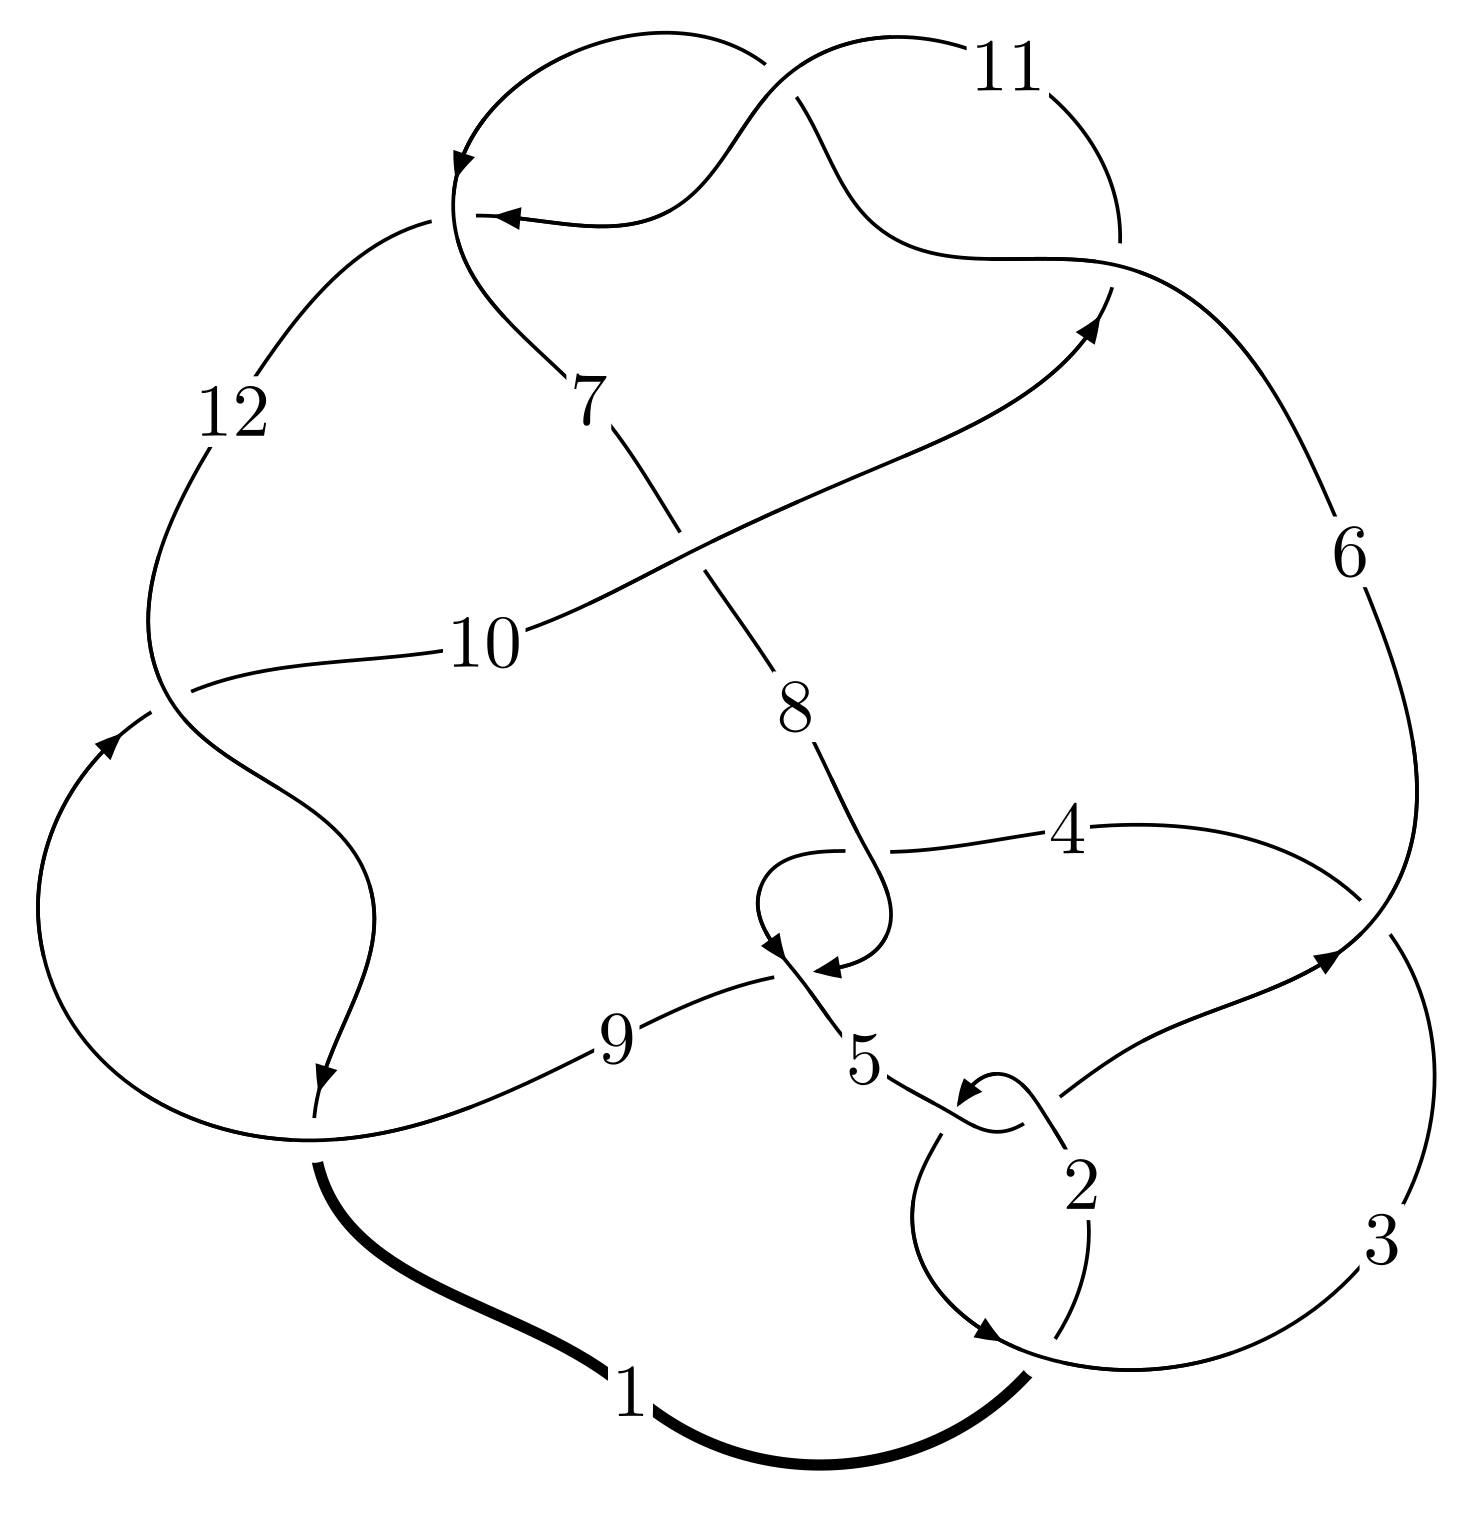
\includegraphics[width=112pt]{../../../GIT/diagram.site/Diagrams/png/2143_12n_0054.png}\\
\ \ \ A knot diagram\footnotemark}&
\allowdisplaybreaks
\textbf{Linearized knot diagam} \\
\cline{2-2}
 &
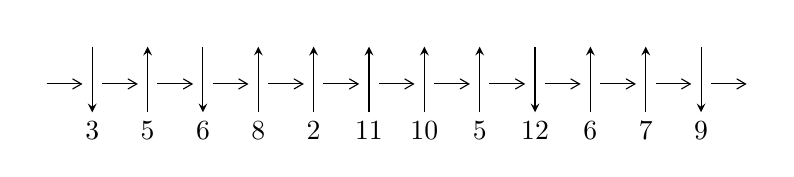
\begin{tikzpicture}[x=20pt, y=17pt]
	% nodes
	\node (C0) at (0, 0) {};
	\node (C1) at (1, 0) {};
	\node (C1U) at (1, +1) {};
	\node (C1D) at (1, -1) {3};

	\node (C2) at (2, 0) {};
	\node (C2U) at (2, +1) {};
	\node (C2D) at (2, -1) {5};

	\node (C3) at (3, 0) {};
	\node (C3U) at (3, +1) {};
	\node (C3D) at (3, -1) {6};

	\node (C4) at (4, 0) {};
	\node (C4U) at (4, +1) {};
	\node (C4D) at (4, -1) {8};

	\node (C5) at (5, 0) {};
	\node (C5U) at (5, +1) {};
	\node (C5D) at (5, -1) {2};

	\node (C6) at (6, 0) {};
	\node (C6U) at (6, +1) {};
	\node (C6D) at (6, -1) {11};

	\node (C7) at (7, 0) {};
	\node (C7U) at (7, +1) {};
	\node (C7D) at (7, -1) {10};

	\node (C8) at (8, 0) {};
	\node (C8U) at (8, +1) {};
	\node (C8D) at (8, -1) {5};

	\node (C9) at (9, 0) {};
	\node (C9U) at (9, +1) {};
	\node (C9D) at (9, -1) {12};

	\node (C10) at (10, 0) {};
	\node (C10U) at (10, +1) {};
	\node (C10D) at (10, -1) {6};

	\node (C11) at (11, 0) {};
	\node (C11U) at (11, +1) {};
	\node (C11D) at (11, -1) {7};

	\node (C12) at (12, 0) {};
	\node (C12U) at (12, +1) {};
	\node (C12D) at (12, -1) {9};
	\node (C13) at (13, 0) {};

	% arrows
	\draw[->,>={angle 60}]
	(C0) edge (C1) (C1) edge (C2) (C2) edge (C3) (C3) edge (C4) (C4) edge (C5) (C5) edge (C6) (C6) edge (C7) (C7) edge (C8) (C8) edge (C9) (C9) edge (C10) (C10) edge (C11) (C11) edge (C12) (C12) edge (C13) ;	\draw[->,>=stealth]
	(C1U) edge (C1D) (C2D) edge (C2U) (C3U) edge (C3D) (C4D) edge (C4U) (C5D) edge (C5U) (C6D) edge (C6U) (C7D) edge (C7U) (C8D) edge (C8U) (C9U) edge (C9D) (C10D) edge (C10U) (C11D) edge (C11U) (C12U) edge (C12D) ;
	\end{tikzpicture} \\
\hhline{~~} \\& 
\textbf{Solving Sequence} \\ \cline{2-2} 
 &
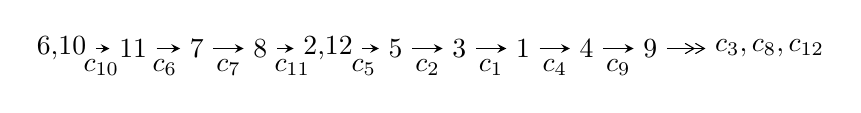
\begin{tikzpicture}[x=23pt, y=7pt]
	% node
	\node (A0) at (-1/8, 0) {6,10};
	\node (A1) at (1, 0) {11};
	\node (A2) at (2, 0) {7};
	\node (A3) at (3, 0) {8};
	\node (A4) at (65/16, 0) {2,12};
	\node (A5) at (41/8, 0) {5};
	\node (A6) at (49/8, 0) {3};
	\node (A7) at (57/8, 0) {1};
	\node (A8) at (65/8, 0) {4};
	\node (A9) at (73/8, 0) {9};
	\node (C1) at (1/2, -1) {$c_{10}$};
	\node (C2) at (3/2, -1) {$c_{6}$};
	\node (C3) at (5/2, -1) {$c_{7}$};
	\node (C4) at (7/2, -1) {$c_{11}$};
	\node (C5) at (37/8, -1) {$c_{5}$};
	\node (C6) at (45/8, -1) {$c_{2}$};
	\node (C7) at (53/8, -1) {$c_{1}$};
	\node (C8) at (61/8, -1) {$c_{4}$};
	\node (C9) at (69/8, -1) {$c_{9}$};
	\node (A10) at (11, 0) {$c_{3},c_{8},c_{12}$};

	% edge
	\draw[->,>=stealth]	
	(A0) edge (A1) (A1) edge (A2) (A2) edge (A3) (A3) edge (A4) (A4) edge (A5) (A5) edge (A6) (A6) edge (A7) (A7) edge (A8) (A8) edge (A9) ;
	\draw[->>,>={angle 60}]	
	(A9) edge (A10);
\end{tikzpicture} \\ 

\end{tabular} \\

\footnotetext{
The image of knot diagram is generated by the software ``\textbf{Draw programme}" developed by Andrew Bartholomew(\url{http://www.layer8.co.uk/maths/draw/index.htm\#Running-draw}), where we modified some parts for our purpose(\url{https://github.com/CATsTAILs/LinksPainter}).
}\phantom \\ \newline 
\centering \textbf{Ideals for irreducible components\footnotemark of $X_{\text{par}}$} 
 
\begin{align*}
I^u_{1}&=\langle 
-2 u^{23}+2 u^{22}+\cdots+2 b-2,\;u^{20}- u^{19}+\cdots+2 a-1,\;u^{24}-3 u^{23}+\cdots- u-1\rangle \\
I^u_{2}&=\langle 
u^4 a+a u+b- a+u,\;u^4 a+u^3 a+u^4-2 u^2 a+2 u^3+a^2- a u- u^2+a-3 u,\;u^5+u^4-2 u^3- u^2+u-1\rangle \\
\\
\end{align*}
\raggedright * 2 irreducible components of $\dim_{\mathbb{C}}=0$, with total 34 representations.\\
\footnotetext{All coefficients of polynomials are rational numbers. But the coefficients are sometimes approximated in decimal forms when there is not enough margin.}
\newpage
\renewcommand{\arraystretch}{1}
\centering \section*{I. $I^u_{1}= \langle -2 u^{23}+2 u^{22}+\cdots+2 b-2,\;u^{20}- u^{19}+\cdots+2 a-1,\;u^{24}-3 u^{23}+\cdots- u-1 \rangle$}
\flushleft \textbf{(i) Arc colorings}\\
\begin{tabular}{m{7pt} m{180pt} m{7pt} m{180pt} }
\flushright $a_{6}=$&$\begin{pmatrix}0\\u\end{pmatrix}$ \\
\flushright $a_{10}=$&$\begin{pmatrix}1\\0\end{pmatrix}$ \\
\flushright $a_{11}=$&$\begin{pmatrix}1\\- u^2\end{pmatrix}$ \\
\flushright $a_{7}=$&$\begin{pmatrix}u\\- u^3+u\end{pmatrix}$ \\
\flushright $a_{8}=$&$\begin{pmatrix}- u^3+2 u\\- u^3+u\end{pmatrix}$ \\
\flushright $a_{2}=$&$\begin{pmatrix}-\frac{1}{2} u^{20}+\frac{1}{2} u^{19}+\cdots-\frac{7}{2} u+\frac{1}{2}\\u^{23}- u^{22}+\cdots+\frac{1}{2} u+1\end{pmatrix}$ \\
\flushright $a_{12}=$&$\begin{pmatrix}- u^2+1\\u^4-2 u^2\end{pmatrix}$ \\
\flushright $a_{5}=$&$\begin{pmatrix}- u^{22}+2 u^{21}+\cdots-\frac{5}{2} u-\frac{3}{2}\\- u^{23}+\frac{3}{2} u^{22}+\cdots-\frac{3}{2} u-1\end{pmatrix}$ \\
\flushright $a_{3}=$&$\begin{pmatrix}- u^{23}+13 u^{21}+\cdots-\frac{7}{2} u-\frac{5}{2}\\-\frac{1}{2} u^{20}+5 u^{18}+\cdots+3 u^2-\frac{1}{2} u\end{pmatrix}$ \\
\flushright $a_{1}=$&$\begin{pmatrix}u^{10}-5 u^8+8 u^6-3 u^4- u^2-1\\- u^{12}+6 u^{10}-12 u^8+8 u^6- u^4+2 u^2\end{pmatrix}$ \\
\flushright $a_{4}=$&$\begin{pmatrix}- u^{23}+13 u^{21}+\cdots-\frac{7}{2} u-\frac{5}{2}\\-4 u^{23}+\frac{11}{2} u^{22}+\cdots-\frac{9}{2} u-3\end{pmatrix}$ \\
\flushright $a_{9}=$&$\begin{pmatrix}u^6-3 u^4+2 u^2+1\\- u^8+4 u^6-4 u^4\end{pmatrix}$\\&\end{tabular}
\flushleft \textbf{(ii) Obstruction class $= -1$}\\~\\
\flushleft \textbf{(iii) Cusp Shapes $= -\frac{5}{2} u^{23}+\frac{7}{2} u^{22}+25 u^{21}-29 u^{20}-\frac{215}{2} u^{19}+83 u^{18}+261 u^{17}-59 u^{16}-\frac{775}{2} u^{15}-\frac{305}{2} u^{14}+325 u^{13}+\frac{601}{2} u^{12}-66 u^{11}-\frac{251}{2} u^{10}-\frac{195}{2} u^9-33 u^8+2 u^7-2 u^6+27 u^5-8 u^4+50 u^3+7 u^2-2 u+\frac{5}{2}$}\\~\\
\newpage\renewcommand{\arraystretch}{1}
\flushleft \textbf{(iv) u-Polynomials at the component}\newline \\
\begin{tabular}{m{50pt}|m{274pt}}
Crossings & \hspace{64pt}u-Polynomials at each crossing \\
\hline $$\begin{aligned}c_{1}\end{aligned}$$&$\begin{aligned}
&u^{24}+2 u^{23}+\cdots-22 u^2+1
\end{aligned}$\\
\hline $$\begin{aligned}c_{2},c_{5}\end{aligned}$$&$\begin{aligned}
&u^{24}+6 u^{23}+\cdots+4 u+1
\end{aligned}$\\
\hline $$\begin{aligned}c_{3}\end{aligned}$$&$\begin{aligned}
&u^{24}-6 u^{23}+\cdots+22568 u+2857
\end{aligned}$\\
\hline $$\begin{aligned}c_{4},c_{8}\end{aligned}$$&$\begin{aligned}
&u^{24}- u^{23}+\cdots+2048 u-1024
\end{aligned}$\\
\hline $$\begin{aligned}c_{6},c_{10},c_{11}\end{aligned}$$&$\begin{aligned}
&u^{24}-3 u^{23}+\cdots- u-1
\end{aligned}$\\
\hline $$\begin{aligned}c_{7}\end{aligned}$$&$\begin{aligned}
&u^{24}+9 u^{23}+\cdots+193 u+37
\end{aligned}$\\
\hline $$\begin{aligned}c_{9},c_{12}\end{aligned}$$&$\begin{aligned}
&u^{24}- u^{23}+\cdots+3 u-1
\end{aligned}$\\
\hline
\end{tabular}\\~\\
\newpage\renewcommand{\arraystretch}{1}
\flushleft \textbf{(v) Riley Polynomials at the component}\newline \\
\begin{tabular}{m{50pt}|m{274pt}}
Crossings & \hspace{64pt}Riley Polynomials at each crossing \\
\hline $$\begin{aligned}c_{1}\end{aligned}$$&$\begin{aligned}
&y^{24}+46 y^{23}+\cdots-44 y+1
\end{aligned}$\\
\hline $$\begin{aligned}c_{2},c_{5}\end{aligned}$$&$\begin{aligned}
&y^{24}+2 y^{23}+\cdots-22 y^2+1
\end{aligned}$\\
\hline $$\begin{aligned}c_{3}\end{aligned}$$&$\begin{aligned}
&y^{24}+90 y^{23}+\cdots+73696224 y+8162449
\end{aligned}$\\
\hline $$\begin{aligned}c_{4},c_{8}\end{aligned}$$&$\begin{aligned}
&y^{24}-55 y^{23}+\cdots+3145728 y+1048576
\end{aligned}$\\
\hline $$\begin{aligned}c_{6},c_{10},c_{11}\end{aligned}$$&$\begin{aligned}
&y^{24}-25 y^{23}+\cdots-7 y+1
\end{aligned}$\\
\hline $$\begin{aligned}c_{7}\end{aligned}$$&$\begin{aligned}
&y^{24}-21 y^{23}+\cdots-29479 y+1369
\end{aligned}$\\
\hline $$\begin{aligned}c_{9},c_{12}\end{aligned}$$&$\begin{aligned}
&y^{24}+43 y^{23}+\cdots-7 y+1
\end{aligned}$\\
\hline
\end{tabular}\\~\\
\newpage\flushleft \textbf{(vi) Complex Volumes and Cusp Shapes}
$$\begin{array}{c|c|c}  
\text{Solutions to }I^u_{1}& \I (\text{vol} + \sqrt{-1}CS) & \text{Cusp shape}\\
 \hline 
\begin{aligned}
u &= -0.576252 + 0.762796 I \\
a &= \phantom{-}0.17468 - 1.56325 I \\
b &= \phantom{-}1.184550 - 0.408250 I\end{aligned}
 & \phantom{-}15.5271 + 1.3395 I & \phantom{-}7.10412 + 0.50033 I \\ \hline\begin{aligned}
u &= -0.576252 - 0.762796 I \\
a &= \phantom{-}0.17468 + 1.56325 I \\
b &= \phantom{-}1.184550 + 0.408250 I\end{aligned}
 & \phantom{-}15.5271 - 1.3395 I & \phantom{-}7.10412 - 0.50033 I \\ \hline\begin{aligned}
u &= -0.514997 + 0.789630 I \\
a &= -1.57008 - 0.30044 I \\
b &= -1.76900 - 0.98677 I\end{aligned}
 & \phantom{-}15.3349 - 6.5027 I & \phantom{-}6.70839 + 4.44626 I \\ \hline\begin{aligned}
u &= -0.514997 - 0.789630 I \\
a &= -1.57008 + 0.30044 I \\
b &= -1.76900 + 0.98677 I\end{aligned}
 & \phantom{-}15.3349 + 6.5027 I & \phantom{-}6.70839 - 4.44626 I \\ \hline\begin{aligned}
u &= \phantom{-}1.225150 + 0.076811 I \\
a &= \phantom{-}0.083295 + 0.422369 I \\
b &= \phantom{-}1.39234 - 0.93644 I\end{aligned}
 & \phantom{-}2.02860 + 0.55793 I & \phantom{-}3.98398 + 0.47568 I \\ \hline\begin{aligned}
u &= \phantom{-}1.225150 - 0.076811 I \\
a &= \phantom{-}0.083295 - 0.422369 I \\
b &= \phantom{-}1.39234 + 0.93644 I\end{aligned}
 & \phantom{-}2.02860 - 0.55793 I & \phantom{-}3.98398 - 0.47568 I \\ \hline\begin{aligned}
u &= \phantom{-}0.386232 + 0.611238 I \\
a &= \phantom{-}0.587872 - 0.504692 I \\
b &= \phantom{-}0.568781 - 0.120868 I\end{aligned}
 & \phantom{-}0.95423 + 1.88035 I & \phantom{-}5.59254 - 3.14019 I \\ \hline\begin{aligned}
u &= \phantom{-}0.386232 - 0.611238 I \\
a &= \phantom{-}0.587872 + 0.504692 I \\
b &= \phantom{-}0.568781 + 0.120868 I\end{aligned}
 & \phantom{-}0.95423 - 1.88035 I & \phantom{-}5.59254 + 3.14019 I \\ \hline\begin{aligned}
u &= -1.368080 + 0.114668 I \\
a &= \phantom{-}0.221757 - 0.722378 I \\
b &= \phantom{-}0.31647 + 2.25463 I\end{aligned}
 & \phantom{-}3.28861 - 3.53789 I & \phantom{-}6.68532 + 4.97474 I \\ \hline\begin{aligned}
u &= -1.368080 - 0.114668 I \\
a &= \phantom{-}0.221757 + 0.722378 I \\
b &= \phantom{-}0.31647 - 2.25463 I\end{aligned}
 & \phantom{-}3.28861 + 3.53789 I & \phantom{-}6.68532 - 4.97474 I\\
 \hline 
 \end{array}$$\newpage$$\begin{array}{c|c|c}  
\text{Solutions to }I^u_{1}& \I (\text{vol} + \sqrt{-1}CS) & \text{Cusp shape}\\
 \hline 
\begin{aligned}
u &= -1.45120 + 0.24568 I \\
a &= -0.508403 + 0.116308 I \\
b &= -1.21041 - 0.93814 I\end{aligned}
 & \phantom{-}6.85595 - 5.06667 I & \phantom{-}9.81977 + 2.58134 I \\ \hline\begin{aligned}
u &= -1.45120 - 0.24568 I \\
a &= -0.508403 - 0.116308 I \\
b &= -1.21041 + 0.93814 I\end{aligned}
 & \phantom{-}6.85595 + 5.06667 I & \phantom{-}9.81977 - 2.58134 I \\ \hline\begin{aligned}
u &= \phantom{-}1.47737 + 0.05442 I \\
a &= -0.580000 - 0.650952 I \\
b &= -1.53636 + 0.50809 I\end{aligned}
 & \phantom{-}6.55976 + 3.21841 I & \phantom{-}9.78805 - 2.36901 I \\ \hline\begin{aligned}
u &= \phantom{-}1.47737 - 0.05442 I \\
a &= -0.580000 + 0.650952 I \\
b &= -1.53636 - 0.50809 I\end{aligned}
 & \phantom{-}6.55976 - 3.21841 I & \phantom{-}9.78805 + 2.36901 I \\ \hline\begin{aligned}
u &= \phantom{-}0.519837\phantom{ +0.000000I} \\
a &= -1.00613\phantom{ +0.000000I} \\
b &= \phantom{-}0.367248\phantom{ +0.000000I}\end{aligned}
 & \phantom{-}1.05585\phantom{ +0.000000I} & \phantom{-}10.2690\phantom{ +0.000000I} \\ \hline\begin{aligned}
u &= -1.50378\phantom{ +0.000000I} \\
a &= \phantom{-}0.695944\phantom{ +0.000000I} \\
b &= \phantom{-}0.281103\phantom{ +0.000000I}\end{aligned}
 & \phantom{-}7.71062\phantom{ +0.000000I} & \phantom{-}11.8740\phantom{ +0.000000I} \\ \hline\begin{aligned}
u &= \phantom{-}0.073930 + 0.488820 I \\
a &= -1.54481 + 0.21964 I \\
b &= -1.121570 + 0.795516 I\end{aligned}
 & -1.23888 + 1.54124 I & -1.90845 - 5.21623 I \\ \hline\begin{aligned}
u &= \phantom{-}0.073930 - 0.488820 I \\
a &= -1.54481 - 0.21964 I \\
b &= -1.121570 - 0.795516 I\end{aligned}
 & -1.23888 - 1.54124 I & -1.90845 + 5.21623 I \\ \hline\begin{aligned}
u &= \phantom{-}1.53161 + 0.28371 I \\
a &= \phantom{-}0.782365 + 0.603573 I \\
b &= \phantom{-}1.95290 - 1.78945 I\end{aligned}
 & -17.4846 + 10.4436 I & \phantom{-}9.58510 - 4.63962 I \\ \hline\begin{aligned}
u &= \phantom{-}1.53161 - 0.28371 I \\
a &= \phantom{-}0.782365 - 0.603573 I \\
b &= \phantom{-}1.95290 + 1.78945 I\end{aligned}
 & -17.4846 - 10.4436 I & \phantom{-}9.58510 + 4.63962 I\\
 \hline 
 \end{array}$$\newpage$$\begin{array}{c|c|c}  
\text{Solutions to }I^u_{1}& \I (\text{vol} + \sqrt{-1}CS) & \text{Cusp shape}\\
 \hline 
\begin{aligned}
u &= \phantom{-}1.55820 + 0.25583 I \\
a &= \phantom{-}0.626457 - 0.749741 I \\
b &= -0.376301 - 0.227538 I\end{aligned}
 & -16.9383 + 2.4136 I & \phantom{-}10.12159 - 0.67000 I \\ \hline\begin{aligned}
u &= \phantom{-}1.55820 - 0.25583 I \\
a &= \phantom{-}0.626457 + 0.749741 I \\
b &= -0.376301 + 0.227538 I\end{aligned}
 & -16.9383 - 2.4136 I & \phantom{-}10.12159 + 0.67000 I \\ \hline\begin{aligned}
u &= -0.349993 + 0.170334 I \\
a &= \phantom{-}2.38196 - 1.38000 I \\
b &= \phantom{-}0.774418 + 0.002185 I\end{aligned}
 & \phantom{-}0.46862 - 2.38365 I & \phantom{-}3.44790 + 2.07617 I \\ \hline\begin{aligned}
u &= -0.349993 - 0.170334 I \\
a &= \phantom{-}2.38196 + 1.38000 I \\
b &= \phantom{-}0.774418 - 0.002185 I\end{aligned}
 & \phantom{-}0.46862 + 2.38365 I & \phantom{-}3.44790 - 2.07617 I\\
 \hline 
 \end{array}$$\newpage\newpage\renewcommand{\arraystretch}{1}
\centering \section*{II. $I^u_{2}= \langle u^4 a+a u+b- a+u,\;u^4 a+u^4+\cdots+a^2+a,\;u^5+u^4-2 u^3- u^2+u-1 \rangle$}
\flushleft \textbf{(i) Arc colorings}\\
\begin{tabular}{m{7pt} m{180pt} m{7pt} m{180pt} }
\flushright $a_{6}=$&$\begin{pmatrix}0\\u\end{pmatrix}$ \\
\flushright $a_{10}=$&$\begin{pmatrix}1\\0\end{pmatrix}$ \\
\flushright $a_{11}=$&$\begin{pmatrix}1\\- u^2\end{pmatrix}$ \\
\flushright $a_{7}=$&$\begin{pmatrix}u\\- u^3+u\end{pmatrix}$ \\
\flushright $a_{8}=$&$\begin{pmatrix}- u^3+2 u\\- u^3+u\end{pmatrix}$ \\
\flushright $a_{2}=$&$\begin{pmatrix}a\\- u^4 a- a u+a- u\end{pmatrix}$ \\
\flushright $a_{12}=$&$\begin{pmatrix}- u^2+1\\u^4-2 u^2\end{pmatrix}$ \\
\flushright $a_{5}=$&$\begin{pmatrix}u^4+u^3-2 u^2+a- u+1\\- u^4 a+u^4+u^2 a- a u-2 u^2+a\end{pmatrix}$ \\
\flushright $a_{3}=$&$\begin{pmatrix}u^4+u^3-2 u^2+a- u+1\\- u^4 a+u^4- a u-2 u^2+a- u\end{pmatrix}$ \\
\flushright $a_{1}=$&$\begin{pmatrix}0\\- u\end{pmatrix}$ \\
\flushright $a_{4}=$&$\begin{pmatrix}u^4+u^3-2 u^2+a- u+1\\- u^4 a+u^4+u^2 a- a u-2 u^2+a\end{pmatrix}$ \\
\flushright $a_{9}=$&$\begin{pmatrix}- u^3+2 u\\- u^3+u\end{pmatrix}$\\&\end{tabular}
\flushleft \textbf{(ii) Obstruction class $= 1$}\\~\\
\flushleft \textbf{(iii) Cusp Shapes $= u^4 a- u^3 a-2 u^2 a+5 u^3+5 a u-9 u+10$}\\~\\
\newpage\renewcommand{\arraystretch}{1}
\flushleft \textbf{(iv) u-Polynomials at the component}\newline \\
\begin{tabular}{m{50pt}|m{274pt}}
Crossings & \hspace{64pt}u-Polynomials at each crossing \\
\hline $$\begin{aligned}c_{1},c_{3},c_{5}\end{aligned}$$&$\begin{aligned}
&(u^2- u+1)^5
\end{aligned}$\\
\hline $$\begin{aligned}c_{2}\end{aligned}$$&$\begin{aligned}
&(u^2+u+1)^5
\end{aligned}$\\
\hline $$\begin{aligned}c_{4},c_{8}\end{aligned}$$&$\begin{aligned}
&u^{10}
\end{aligned}$\\
\hline $$\begin{aligned}c_{6}\end{aligned}$$&$\begin{aligned}
&(u^5- u^4-2 u^3+u^2+u+1)^2
\end{aligned}$\\
\hline $$\begin{aligned}c_{7}\end{aligned}$$&$\begin{aligned}
&(u^5+3 u^4+4 u^3+u^2- u-1)^2
\end{aligned}$\\
\hline $$\begin{aligned}c_{9}\end{aligned}$$&$\begin{aligned}
&(u^5+u^4+2 u^3+u^2+u+1)^2
\end{aligned}$\\
\hline $$\begin{aligned}c_{10},c_{11}\end{aligned}$$&$\begin{aligned}
&(u^5+u^4-2 u^3- u^2+u-1)^2
\end{aligned}$\\
\hline $$\begin{aligned}c_{12}\end{aligned}$$&$\begin{aligned}
&(u^5- u^4+2 u^3- u^2+u-1)^2
\end{aligned}$\\
\hline
\end{tabular}\\~\\
\newpage\renewcommand{\arraystretch}{1}
\flushleft \textbf{(v) Riley Polynomials at the component}\newline \\
\begin{tabular}{m{50pt}|m{274pt}}
Crossings & \hspace{64pt}Riley Polynomials at each crossing \\
\hline $$\begin{aligned}c_{1},c_{2},c_{3}\\c_{5}\end{aligned}$$&$\begin{aligned}
&(y^2+y+1)^5
\end{aligned}$\\
\hline $$\begin{aligned}c_{4},c_{8}\end{aligned}$$&$\begin{aligned}
&y^{10}
\end{aligned}$\\
\hline $$\begin{aligned}c_{6},c_{10},c_{11}\end{aligned}$$&$\begin{aligned}
&(y^5-5 y^4+8 y^3-3 y^2- y-1)^2
\end{aligned}$\\
\hline $$\begin{aligned}c_{7}\end{aligned}$$&$\begin{aligned}
&(y^5- y^4+8 y^3-3 y^2+3 y-1)^2
\end{aligned}$\\
\hline $$\begin{aligned}c_{9},c_{12}\end{aligned}$$&$\begin{aligned}
&(y^5+3 y^4+4 y^3+y^2- y-1)^2
\end{aligned}$\\
\hline
\end{tabular}\\~\\
\newpage\flushleft \textbf{(vi) Complex Volumes and Cusp Shapes}
$$\begin{array}{c|c|c}  
\text{Solutions to }I^u_{2}& \I (\text{vol} + \sqrt{-1}CS) & \text{Cusp shape}\\
 \hline 
\begin{aligned}
u &= \phantom{-}1.21774\phantom{ +0.000000I} \\
a &= -0.410598 + 0.711177 I \\
b &= -0.22546 - 1.71868 I\end{aligned}
 & \phantom{-}2.40108 - 2.02988 I & \phantom{-}6.62546 + 2.50057 I \\ \hline\begin{aligned}
u &= \phantom{-}1.21774\phantom{ +0.000000I} \\
a &= -0.410598 - 0.711177 I \\
b &= -0.22546 + 1.71868 I\end{aligned}
 & \phantom{-}2.40108 + 2.02988 I & \phantom{-}6.62546 - 2.50057 I \\ \hline\begin{aligned}
u &= \phantom{-}0.309916 + 0.549911 I \\
a &= -1.58413 + 0.01647 I \\
b &= -1.51295 + 0.11095 I\end{aligned}
 & \phantom{-}0.329100 - 0.499304 I & \phantom{-}5.04069 - 0.50981 I \\ \hline\begin{aligned}
u &= \phantom{-}0.309916 + 0.549911 I \\
a &= \phantom{-}0.80632 + 1.36366 I \\
b &= \phantom{-}0.863922 + 0.161516 I\end{aligned}
 & \phantom{-}0.32910 + 3.56046 I & \phantom{-}2.53179 - 8.01848 I \\ \hline\begin{aligned}
u &= \phantom{-}0.309916 - 0.549911 I \\
a &= -1.58413 - 0.01647 I \\
b &= -1.51295 - 0.11095 I\end{aligned}
 & \phantom{-}0.329100 + 0.499304 I & \phantom{-}5.04069 + 0.50981 I \\ \hline\begin{aligned}
u &= \phantom{-}0.309916 - 0.549911 I \\
a &= \phantom{-}0.80632 - 1.36366 I \\
b &= \phantom{-}0.863922 - 0.161516 I\end{aligned}
 & \phantom{-}0.32910 - 3.56046 I & \phantom{-}2.53179 + 8.01848 I \\ \hline\begin{aligned}
u &= -1.41878 + 0.21917 I \\
a &= \phantom{-}0.252108 + 0.649344 I \\
b &= -0.291925 - 0.343564 I\end{aligned}
 & \phantom{-}5.87256 - 2.37095 I & \phantom{-}9.19707 + 1.05452 I \\ \hline\begin{aligned}
u &= -1.41878 + 0.21917 I \\
a &= \phantom{-}0.436295 - 0.543004 I \\
b &= \phantom{-}2.16641 + 1.32455 I\end{aligned}
 & \phantom{-}5.87256 - 6.43072 I & \phantom{-}6.60498 + 6.63374 I \\ \hline\begin{aligned}
u &= -1.41878 - 0.21917 I \\
a &= \phantom{-}0.252108 - 0.649344 I \\
b &= -0.291925 + 0.343564 I\end{aligned}
 & \phantom{-}5.87256 + 2.37095 I & \phantom{-}9.19707 - 1.05452 I \\ \hline\begin{aligned}
u &= -1.41878 - 0.21917 I \\
a &= \phantom{-}0.436295 + 0.543004 I \\
b &= \phantom{-}2.16641 - 1.32455 I\end{aligned}
 & \phantom{-}5.87256 + 6.43072 I & \phantom{-}6.60498 - 6.63374 I\\
 \hline 
 \end{array}$$\newpage
\newpage\renewcommand{\arraystretch}{1}
\centering \section*{ III. u-Polynomials}
\begin{tabular}{m{50pt}|m{274pt}}
Crossings & \hspace{64pt}u-Polynomials at each crossing \\
\hline $$\begin{aligned}c_{1}\end{aligned}$$&$\begin{aligned}
&((u^2- u+1)^5)(u^{24}+2 u^{23}+\cdots-22 u^2+1)
\end{aligned}$\\
\hline $$\begin{aligned}c_{2}\end{aligned}$$&$\begin{aligned}
&((u^2+u+1)^5)(u^{24}+6 u^{23}+\cdots+4 u+1)
\end{aligned}$\\
\hline $$\begin{aligned}c_{3}\end{aligned}$$&$\begin{aligned}
&((u^2- u+1)^5)(u^{24}-6 u^{23}+\cdots+22568 u+2857)
\end{aligned}$\\
\hline $$\begin{aligned}c_{4},c_{8}\end{aligned}$$&$\begin{aligned}
&u^{10}(u^{24}- u^{23}+\cdots+2048 u-1024)
\end{aligned}$\\
\hline $$\begin{aligned}c_{5}\end{aligned}$$&$\begin{aligned}
&((u^2- u+1)^5)(u^{24}+6 u^{23}+\cdots+4 u+1)
\end{aligned}$\\
\hline $$\begin{aligned}c_{6}\end{aligned}$$&$\begin{aligned}
&((u^5- u^4-2 u^3+u^2+u+1)^2)(u^{24}-3 u^{23}+\cdots- u-1)
\end{aligned}$\\
\hline $$\begin{aligned}c_{7}\end{aligned}$$&$\begin{aligned}
&((u^5+3 u^4+4 u^3+u^2- u-1)^2)(u^{24}+9 u^{23}+\cdots+193 u+37)
\end{aligned}$\\
\hline $$\begin{aligned}c_{9}\end{aligned}$$&$\begin{aligned}
&((u^5+u^4+2 u^3+u^2+u+1)^2)(u^{24}- u^{23}+\cdots+3 u-1)
\end{aligned}$\\
\hline $$\begin{aligned}c_{10},c_{11}\end{aligned}$$&$\begin{aligned}
&((u^5+u^4-2 u^3- u^2+u-1)^2)(u^{24}-3 u^{23}+\cdots- u-1)
\end{aligned}$\\
\hline $$\begin{aligned}c_{12}\end{aligned}$$&$\begin{aligned}
&((u^5- u^4+2 u^3- u^2+u-1)^2)(u^{24}- u^{23}+\cdots+3 u-1)
\end{aligned}$\\
\hline
\end{tabular}\newpage\renewcommand{\arraystretch}{1}
\centering \section*{ IV. Riley Polynomials}
\begin{tabular}{m{50pt}|m{274pt}}
Crossings & \hspace{64pt}Riley Polynomials at each crossing \\
\hline $$\begin{aligned}c_{1}\end{aligned}$$&$\begin{aligned}
&((y^2+y+1)^5)(y^{24}+46 y^{23}+\cdots-44 y+1)
\end{aligned}$\\
\hline $$\begin{aligned}c_{2},c_{5}\end{aligned}$$&$\begin{aligned}
&((y^2+y+1)^5)(y^{24}+2 y^{23}+\cdots-22 y^2+1)
\end{aligned}$\\
\hline $$\begin{aligned}c_{3}\end{aligned}$$&$\begin{aligned}
&((y^2+y+1)^5)(y^{24}+90 y^{23}+\cdots+7.36962\times10^{7} y+8162449)
\end{aligned}$\\
\hline $$\begin{aligned}c_{4},c_{8}\end{aligned}$$&$\begin{aligned}
&y^{10}(y^{24}-55 y^{23}+\cdots+3145728 y+1048576)
\end{aligned}$\\
\hline $$\begin{aligned}c_{6},c_{10},c_{11}\end{aligned}$$&$\begin{aligned}
&((y^5-5 y^4+8 y^3-3 y^2- y-1)^2)(y^{24}-25 y^{23}+\cdots-7 y+1)
\end{aligned}$\\
\hline $$\begin{aligned}c_{7}\end{aligned}$$&$\begin{aligned}
&((y^5- y^4+8 y^3-3 y^2+3 y-1)^2)(y^{24}-21 y^{23}+\cdots-29479 y+1369)
\end{aligned}$\\
\hline $$\begin{aligned}c_{9},c_{12}\end{aligned}$$&$\begin{aligned}
&((y^5+3 y^4+4 y^3+y^2- y-1)^2)(y^{24}+43 y^{23}+\cdots-7 y+1)
\end{aligned}$\\
\hline
\end{tabular}
\vskip 2pc
\end{document}